\section{子图,图的运算,图同构}
\subsection{子图}
\begin{definition}
%@see: 《离散数学》(邓辉文) P171 定义6-10
设\(G = (V,E)\)和\(H = (W,F)\)都是图.
若\(W \subseteq V\)且\(F \subseteq E\),
则称“\(H\)是\(G\)的一个\DefineConcept{子图}(subgraph)”
%@see: 《Graph Theory》(Reinhard Diestel) P3
“\(G\)是\(H\)的一个\DefineConcept{超图}(supergraph)”,
记作\(H \subseteq G\).
\end{definition}

\begin{definition}
%@see: 《Graph Theory》(Reinhard Diestel) P3
设图\(H \subseteq G\)且\(H \neq G\),
则称“\(H\)是\(G\)的一个\DefineConcept{真子图}(\(H\) is a \emph{proper subgraph} of \(G\))”,
记作\(H \subset G\).
\end{definition}

\begin{definition}
%@see: 《离散数学》(邓辉文) P172 定义6-10
设\(H = (W,F)\)是\(G = (V,E)\)的子图.
如果\(W = V\),
则称“\(H\)是\(G\)的一个\DefineConcept{生成子图}(spanning subgraph)”.
\end{definition}

%@see: 《离散数学》(邓辉文) P172
常见的4种产生\(G = (V,E)\)的子图的方式:
\begin{center}
\begin{tblr}{p{2cm}p{13cm}}
	{\(G[W]\)法} &
	设\(W \subseteq V\).
	以\(W\)为顶点集,
	以两端点均属于\(W\)的所有边为边集,
	构成的子图,
	称为\DefineConcept{由\(W\)导出的子图}(induced subgraph by \(W\)),
	记作\(G[W]\).
	\\
	{\(G-W\)法} &
	设\(W \subseteq V\).
	将由\(V-W\)导出的子图\(G[V-W]\)
	记作\(G-W\).
	\\
	{\(G[F]\)法} &
	设\(F \subseteq E\).
	以\(F\)为边集,
	以\(F\)中边的所有端点为顶点集,
	构成的子图,
	称为\DefineConcept{由\(F\)导出的子图}(induced subgraph by \(F\)),
	记作\(G[F]\).
	\\
	{\(G-F\)法} &
	设\(F \subseteq E\).
	将由\(E-F\)导出的子图\(G[E-F]\)
	记作\(G-F\).
	\\
\end{tblr}
\end{center}

\begin{proposition}
%@see: 《离散数学》(邓辉文) P172
设\(G = (V,E)\)是\(n\)阶简单无向图,
则\(G\)的补图为\(\overline{G} = K_n - E\).
\end{proposition}

我们除了可以产生子图以外,还可以反过来,在图\(G = (V,E)\)的基础上,
通过在\(V\)中某些顶点之间增加一些新的边\(U\),得到一个更大的图\(G + U\).

\subsection{图的运算}
图的运算就是通过一些操作,产生新的图.
上一小节讨论的子图的产生方法,在本质上是图的一种运算,但它只涉及一个图.
本章第一节讨论的补图的计算方法,同样在本质上是图的一种运算,而且它涉及两个图.

下面我们来讨论两个图之间的运算.
\begin{definition}
%@see: 《离散数学》(邓辉文) P173 定义6-11
设\(G_1 = (V_1,E_1)\)和\(G_2 = (V_2,E_2)\)都是无向图(或有向图).
\begin{itemize}
	\item 把满足\[
		E = E_1 \cup E_2,
		\qquad
		V = V_1 \cup V_2
	\]的图\(G = (V,E)\)
	称为“\(G_1\)与\(G_2\)的\DefineConcept{并}”,
	记作\(G_1 \cup G_2\).

	\item 把满足\[
		E = E_1 \cap E_2,
		\qquad
		V = V_1 \cap V_2
	\]的图\(G = (V,E)\)
	称为“\(G_1\)与\(G_2\)的\DefineConcept{交}”,
	记作\(G_1 \cap G_2\).

	\item 把满足\[
		E = E_1 - E_2,
		\qquad
		V = V_1
	\]的图\(G = (V,E)\)
	称为“\(G_1\)与\(G_2\)的\DefineConcept{差}”,
	记作\(G_1 - G_2\).

	\item 把满足\[
		E = E_1 \symdiff E_2,
		\qquad
		V = V_1 \cup V_2
	\]的图\(G = (V,E)\)
	称为“\(G_1\)与\(G_2\)的\DefineConcept{对称差}”
	或“\(G_1\)与\(G_2\)的\DefineConcept{环和}(ring sum)”,
	记作\(G_1 \symdiff G_2\).
\end{itemize}
\end{definition}

\subsection{图同构}
由于图的拓扑不变性,
两个看上去不同的图,有可能本质上是同一个图,
这就是图同构的问题.

\begin{definition}
%@see: 《离散数学》(邓辉文) P173 定义6-12
%@see: 《Graph Theory》(Reinhard Diestel) P3
设\(G_1 = (V_1,E_1)\)和\(G_2 = (V_2,E_2)\)都是无向图(或有向图).
如果存在双射\(\rho,\sigma\)满足\begin{equation*}
	(\forall u_1,v_1 \in V_1)
	(\forall e_1 \in E_1)
	\left[
		\text{$e_1$与$u_1,v_1$是关联的}
		\iff
		\text{$\sigma(v_1)$与$\rho(u_1),\rho(v_1)$是关联的}
	\right],
\end{equation*}
则称“图\(G_1\)与\(G_2\) \DefineConcept{同构}%
(\(G_1\) and \(G_2\) are \emph{isomorphic})”,
记作\(G_1 \Isomorphism G_2\).
\end{definition}

由定义可知,两个图同构,当且仅当这两个图的顶点与边分别一一对应,并且保持顶点与边的关联关系.
或者更直观地说,两个图同构,是指其中一个图仅经过顶点的位移和边的形变这两种变换,就可以变为另一个图.

容易看出,
\cref{figure:图论.补图.原图1,figure:图论.补图.补图1} 中的两个图是同构的,
\cref{figure:图论.正则图1,figure:图论.K33} 中的两个图是不同构的.

\begin{figure}[hbt]
%@see: 《离散数学》(邓辉文) P173 图6-17(b)
	\centering
	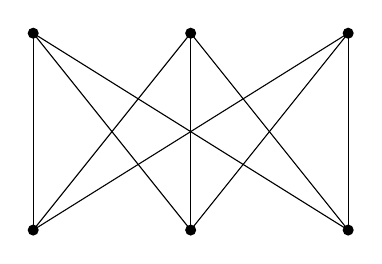
\begin{tikzpicture}
		\fill(0,0)coordinate(A1)circle(2pt);
		\fill(2,0)coordinate(A2)circle(2pt);
		\fill(4,0)coordinate(A3)circle(2pt);
		\fill(0,2.5)coordinate(B1)circle(2pt);
		\fill(2,2.5)coordinate(B2)circle(2pt);
		\fill(4,2.5)coordinate(B3)circle(2pt);
		\foreach \j in {1,...,3} {
			\foreach \k in {1,...,3} {
				\draw(A\j)--(B\k);
			}
		}
	\end{tikzpicture}
	\caption{}
	\label{figure:图论.K33}
\end{figure}

在判断两个有向图是否同构时,要特别注意边的方向的一致性.

\begin{definition}
%@see: 《离散数学》(邓辉文) P175 习题6.3 7.
若一个简单无向图\(G\)与它的补图\(\overline{G}\)同构,
则称“\(G\)是一个\DefineConcept{自补图}”.
\end{definition}

\begin{example}
%@see: 《离散数学》(邓辉文) P175 习题6.3 7.(2)
设\(G\)是\(n\)阶自补图.
证明:\(K_n\)的边数是偶数.
%TODO proof
\end{example}

\begin{example}
%@see: 《离散数学》(邓辉文) P175 习题6.3 7.(3)
设\(G\)是\(n\ (n\geq2)\)阶自补图.
证明:存在正整数\(k\)使得\(n=4k\)或\(n=4k+1\).
%TODO proof
\end{example}

2015年,芝加哥大学 Babai 教授给出了在拟多项式时间复杂度内判定两个图同构的算法.
%TODO 看一下参考文献

\begin{conjecture}[乌拉姆猜想(1929)]
%@see: 《离散数学》(邓辉文) P174 乌拉姆(Ulam)猜想(1929)
设\(G_1,G_2\)都是简单无向图,
\(V(G_1) = \{\AutoTuple{v}{n}\},
V(G_2) = \{\AutoTuple{w}{n}\}\).
若对于任意\(i=1,2,\dotsc,n\)均有\(G_1 - v_i \Isomorphism G_2 - w_i\),
则\(G_1 \Isomorphism G_2\).
%@see: https://mathworld.wolfram.com/UlamsConjecture.html
\end{conjecture}
